% =============================================================================
%  Heterogeneity-Driven Expansion and Synchronization Collapse
%  in Coupled Ornstein-Uhlenbeck Systems
%
%  REVISED VERSION (v2), September 2026.
%
%  PROVENANCE NOTICE.  The LaTeX source of version 1 (Zenodo, August 2026) was
%  not preserved and could not be located.  This file is a RECONSTRUCTION of
%  that manuscript from the deposited PDF, followed by the revisions listed in
%  Section 0 and in CHANGELOG.md.  It is not the original source file.  The
%  mathematical content of v1 was transcribed statement by statement and
%  re-checked symbolically; the prose is reconstructed and may differ from v1
%  in wording, line breaks, and equation numbering.
% =============================================================================

\documentclass[11pt]{article}

\usepackage[letterpaper,margin=1in]{geometry}
\usepackage{amsmath,amssymb,amsthm}
\usepackage{graphicx}
\usepackage{booktabs}
\usepackage[T1]{fontenc}
\usepackage[utf8]{inputenc}
\usepackage{microtype}
\usepackage[colorlinks=true,linkcolor=blue,citecolor=blue,urlcolor=blue]{hyperref}

\theoremstyle{plain}
\newtheorem{theorem}{Theorem}
\newtheorem{proposition}{Proposition}
\newtheorem{corollary}{Corollary}
\theoremstyle{remark}
\newtheorem{remark}{Remark}

\newcommand{\Var}{\operatorname{Var}}
\newcommand{\tr}{\operatorname{tr}}
\newcommand{\I}{I}
\newcommand{\rA}{r_A^{*}}
\newcommand{\rD}{r_D^{*}}

\title{Heterogeneity-Driven Expansion and Synchronization Collapse\\
in Coupled Ornstein--Uhlenbeck Systems}
\author{Elias De Jes\'us\\
Independent Researcher\\
ORCID: 0009-0007-0190-9143}
\date{Version 2 --- September 2026\\[2pt]
\small (Version 1: August 2026)}

\begin{document}
\maketitle

\begin{abstract}
We study two diffusively coupled Ornstein--Uhlenbeck processes with unequal noise amplitudes
and analyze the stationary covariance matrix $\Sigma(\kappa)$ exactly, through the continuous
Lyapunov equation, as a function of the coupling strength $\kappa$. Three scalar functionals of
$\Sigma(\kappa)$ are considered: the residual variance $D(\kappa)=\Var(X\mid Y)$, the Gaussian
mutual information $C(\kappa)=\I(X;Y)$, and the stationary covariance-volume proxy
$A(\kappa)=\det\Sigma(\kappa)$. We prove that for arbitrary positive relaxation rates and noise
amplitudes, $A'(0)<0$, so infinitesimal diffusive coupling always initially contracts the
stationary covariance volume. In the equal-relaxation case, we then prove the exact threshold
\[
  \sup_{\kappa>0}A(\kappa)>A(0)
  \iff
  \max\!\left(\frac{\sigma_1}{\sigma_2},\frac{\sigma_2}{\sigma_1}\right)>3+2\sqrt{2}.
\]
When this threshold is exceeded, the enhancement occurs on a bounded interval whose two
endpoints satisfy the exact reciprocal identity $\kappa_1\kappa_2=1$. A second exact threshold,
$2+\sqrt{3}$, governs whether the conditional residual variance $D(\kappa)$ can exceed its
uncoupled value. Thus distinct legitimate measures of relational structure acquire enhancement
at different heterogeneity scales. We also prove that Gaussian coherence $C(\kappa)$ increases
strictly with coupling, while in the strong-coupling limit $\rho\to1$, $D(\kappa)\to0$,
$A(\kappa)\to0$, with explicit asymptotic rates.

This version adds three things to the August 2026 version. First, the two thresholds are shown
to share a single reciprocal structure: both are roots of $x^2-cx+1=0$, with $c=6$ for the
volume threshold and $c=4$ for the residual threshold, and at the coupling where the volume
enhancement region closes the eigenvalue ratio of $\Sigma$ equals $(2+\sqrt{3})^2$ exactly.
Second, the central algebraic statements have been machine-checked in Lean~4 with mathlib.
Third, several statements of the first version have been corrected or sharpened, in particular
the description of the normal-mode reduction, in which heterogeneous noise makes the two
normal modes \emph{correlated} rather than independent. The results are specific to this
linear-Gaussian model and are not claimed to establish a general principle for nonlinear,
biological, cognitive, or social systems.
\end{abstract}

\section*{0. Status of this version}
\addcontentsline{toc}{section}{0. Status of this version}

\paragraph{Reconstruction notice.} The LaTeX source of version~1 was not preserved. This
document was reconstructed from the deposited PDF of version~1 and then revised. Every
displayed equation of version~1 was transcribed and re-verified symbolically before being
carried over; the surrounding prose is a reconstruction and differs from version~1 in wording
and in equation and section numbering. Readers wanting the exact text of version~1 should
consult that version of the record, which remains available and is not superseded as a record
of what was written in August 2026.

\paragraph{What changed.} A full list is in \texttt{CHANGELOG.md} accompanying this version.
The substantive changes are:

\begin{enumerate}\itemsep2pt
\item A new Section~\ref{sec:reciprocal} on the reciprocal structure shared by the two
  thresholds and on a cross-threshold identity relating them at the merger coupling.
\item A new Section~\ref{sec:lean} reporting a machine-checked formalization of the central
  algebraic statements in Lean~4 with mathlib, together with an explicit statement of which
  results of this paper are \emph{not} formalized.
\item A correction, in Section~\ref{sec:modes}, to the treatment of the normal-mode
  decomposition: the symmetric and antisymmetric modes have uncorrelated forcing only in the
  homogeneous case $\sigma_1=\sigma_2$. For $\sigma_1\neq\sigma_2$ they are driven by
  correlated noise, and that correlation is exactly what produces the enhancement regime.
\item A sharpening of terminology around the word \emph{synchronization}
  (Section~\ref{sec:strong}, Remark~\ref{rem:synch}).
\item An explicit distinction between the amplitude ratio $r$ and the variance ratio $t=r^2$,
  and between their respective reciprocal invariants (Section~\ref{sec:ratios}).
\item Strengthened limitations (Section~\ref{sec:limitations}).
\item A one-paragraph pointer to a companion formalization of a general two-mode reduction
  that contains the present volume threshold as a special case
  (Section~\ref{sec:companion}).
\item A fuller statement of AI assistance (Acknowledgments).
\end{enumerate}

No result of version~1 is retracted. The thresholds $3+2\sqrt2$ and $2+\sqrt3$, the identity
$\kappa_1\kappa_2=1$, the sign of $A'(0)$, the monotonicity of $C$, and the strong-coupling
asymptotics all stand as stated, and several of them now stand as machine-checked statements
of exact real algebra.

\section{Introduction}

Coupling two dynamical systems can either enlarge or reduce the range of configurations
occupied by the joint system. At one limit, weakly coupled systems remain nearly independent.
At the opposite limit, sufficiently strong diffusive coupling can drive the components toward a
common synchronization manifold, reducing their effectively independent degrees of freedom.

A natural intermediate question is therefore whether coupling can increase the joint
configuration volume before synchronization eventually reduces it.

The difficulty is that terms such as ``coherence,'' ``distinction,'' ``richness,'' and
``accessibility'' can refer to mathematically different objects. In the present paper we avoid
treating them as interchangeable. Instead, we analyze a minimal model in which several such
quantities can be calculated exactly: two diffusively coupled Ornstein--Uhlenbeck (OU)
processes with independent additive Gaussian noise \cite{UhlenbeckOrnstein1930,Gardiner2004}.

Because the system is linear and Gaussian, its stationary dynamics are fully characterized by a
$2\times2$ covariance matrix $\Sigma(\kappa)$. This permits three related but distinct
quantities to be studied explicitly:
\begin{align}
  D(\kappa) &= \Var(X\mid Y), \label{eq:D}\\
  C(\kappa) &= \I(X;Y), \label{eq:C}\\
  A(\kappa) &= \det\Sigma(\kappa). \label{eq:A}
\end{align}

The principal result is an exact threshold for the last quantity. For equal intrinsic
relaxation rates, the stationary covariance volume can exceed its uncoupled value at some
finite coupling strength if and only if the noise-amplitude ratio exceeds $3+2\sqrt2$.

A second exact threshold, $2+\sqrt3$, controls whether the residual variance $D(\kappa)$ can
exceed its uncoupled value. Thus even within this simplest solvable setting, different
legitimate measures of relational structure do not acquire enhancement at the same parameter
value.

The results should be read narrowly. We establish an exact property of a two-dimensional linear
stochastic model. We do not infer from it a general law of heterogeneous interaction.

\section{Relation to Existing Work}

The present model lies at the intersection of several established literatures.

\paragraph{Synchronization.} The reduction of independent degrees of freedom under strong
coupling is part of the broad theory of synchronization of coupled dynamical systems
\cite{PikovskyEtAl2001}. For networks of identical oscillators, the master-stability framework
of Pecora and Carroll separates longitudinal and transverse perturbation modes relative to a
synchronization manifold \cite{PecoraCarroll1998}. Generalized synchronization extends this
idea to functional relations between nonidentical systems
\cite{RulkovEtAl1995,KocarevParlitz1996,AbarbanelEtAl1996}. As emphasized in
Remark~\ref{rem:synch} below, the present paper borrows the \emph{geometry} of that
decomposition --- a longitudinal and a transverse mode relative to $x=y$ --- but not its
stability-theoretic content: our system is linear and always has a unique stationary
distribution, so no master stability function is involved and nothing here is
synchronization in the sense of those works.

\paragraph{Amplitude and oscillation death.} Strong coupling can also suppress oscillatory
dynamics entirely in nonlinear oscillator systems \cite{AronsonEtAl1990}. That mechanism is
distinct from the present one: our OU system possesses no limit cycle, and the strong-coupling
collapse concerns the stationary covariance ellipse approaching a lower-dimensional line rather
than the disappearance of an oscillation.

\paragraph{Heterogeneous OU processes.} Stationary covariance matrices of coupled heterogeneous
OU processes have been studied directly through Sylvester--Lyapunov equations. Barucca
investigated localization phenomena in covariance matrices of heterogeneous OU processes
\cite{Barucca2014}, and Ferreira, Metz, and Barucca subsequently developed a random-matrix
ensemble for covariance matrices of OU systems with heterogeneous temperatures
\cite{FerreiraMetzBarucca2025}. Godr\`eche and Luck give exact stationary results for coupled
linear Langevin systems driven at two temperatures \cite{GodrecheLuck2019}, and the Brownian
gyrator literature \cite{FilligerReimann2007,DotsenkoEtAl2013} studies the same two-temperature
structure in a linear planar model. These works provide the closest mathematical setting to the
present calculation, and the modal solution used in Section~\ref{sec:modes} is standard in
them.

We did not identify in the literature examined the specific two-node enhancement thresholds
$3+2\sqrt2$ and $2+\sqrt3$, nor the cross-threshold identity of Section~\ref{sec:reciprocal}.
No claim of priority is made beyond the scope of that search; a fuller account of what was
searched, and of which ingredients here are standard, is kept with the formalization
repository.

\paragraph{Information theory.} For jointly Gaussian variables, mutual information, conditional
variance, covariance determinants, and differential entropy have standard closed forms
\cite{CoverThomas2005,Lauritzen1996}. We use these exact identities directly. The determinant
$\det\Sigma$ as a scalar summary of a covariance matrix is Wilks's generalized variance
\cite{Wilks1932}.

\paragraph{Viability language.} Constraint-based formulations of persistence are central to
viability theory \cite{Aubin1991}. A set of coupling strengths satisfying simultaneous
conditions on $D$, $C$, and $A$ can be viewed informally as a feasible parameter region. We do
not, however, claim that the parameter-space construction used later is itself a viability
kernel in the strict state-space sense.

\paragraph{Synergetics.} The elimination of fast transverse degrees of freedom under strong
coupling has a conceptual relation to slaving and dimension reduction in synergetics
\cite{Haken1983}. The analogy is structural rather than an identification of mechanisms.

\section{Coupled Ornstein--Uhlenbeck Model}

Consider
\begin{align}
  dx &= -\bigl(a_1x+\kappa(y-x)\bigr)\,dt+\sigma_1\,dW_1, \label{eq:sde1}\\
  dy &= -\bigl(a_2y+\kappa(x-y)\bigr)\,dt+\sigma_2\,dW_2, \label{eq:sde2}
\end{align}
with $a_1,a_2>0$, $\sigma_1,\sigma_2>0$, $\kappa\ge0$, and independent standard Brownian
motions $W_1,W_2$.

Writing $Z=(x,y)^{\top}$, the dynamics become
\begin{equation}
  dZ = MZ\,dt + B\,dW, \label{eq:linear}
\end{equation}
where
\begin{equation}
  M=\begin{pmatrix}-(a_1+\kappa)&\kappa\\ \kappa&-(a_2+\kappa)\end{pmatrix},
  \qquad
  B=\begin{pmatrix}\sigma_1&0\\ 0&\sigma_2\end{pmatrix}. \label{eq:MB}
\end{equation}

The noise covariance is $Q=BB^{\top}=\operatorname{diag}(\sigma_1^2,\sigma_2^2)$. The trace and
determinant of the drift matrix are
\[
  \tr M=-(a_1+a_2+2\kappa)<0,
  \qquad
  \det M=a_1a_2+\kappa(a_1+a_2)>0,
\]
so $M$ is Hurwitz for all allowed parameter values.

\begin{proposition}[Stationary Gaussian state]\label{prop:stationary}
For every $a_1,a_2,\sigma_1,\sigma_2>0$ and $\kappa\ge0$, the system possesses a unique
zero-mean stationary Gaussian distribution whose covariance matrix $\Sigma$ solves
\begin{equation}
  M\Sigma+\Sigma M^{\top}=-Q. \label{eq:lyapunov}
\end{equation}
\end{proposition}

This is the standard stationary covariance relation for a linear stochastic system with Hurwitz
drift matrix \cite{Gardiner2004,Vatiwutipong2019}.

\section{Exact Stationary Covariance}

Write
\[
  \Sigma=\begin{pmatrix}\Sigma_{xx}&\Sigma_{xy}\\ \Sigma_{xy}&\Sigma_{yy}\end{pmatrix}.
\]
Solving Eq.~\eqref{eq:lyapunov} gives the following exact expressions.

\begin{proposition}[Exact stationary covariance]\label{prop:cov}
Define
\begin{equation}
  \Delta = a_1^2a_2+a_1^2\kappa+a_1a_2^2+4a_1a_2\kappa+2a_1\kappa^2+a_2^2\kappa+2a_2\kappa^2.
  \label{eq:Delta}
\end{equation}
Then
\begin{align}
  \Sigma_{xx} &= \frac{a_1a_2\sigma_1^2+a_1\kappa\sigma_1^2+a_2^2\sigma_1^2
    +3a_2\kappa\sigma_1^2+\kappa^2\sigma_1^2+\kappa^2\sigma_2^2}{2\Delta}, \label{eq:Sxx}\\[2pt]
  \Sigma_{yy} &= \frac{a_1^2\sigma_2^2+a_1a_2\sigma_2^2+3a_1\kappa\sigma_2^2
    +a_2\kappa\sigma_2^2+\kappa^2\sigma_1^2+\kappa^2\sigma_2^2}{2\Delta}, \label{eq:Syy}\\[2pt]
  \Sigma_{xy} &= \frac{\kappa\bigl(a_1\sigma_2^2+a_2\sigma_1^2+\kappa\sigma_1^2
    +\kappa\sigma_2^2\bigr)}{2\Delta}. \label{eq:Sxy}
\end{align}
Consequently,
\begin{equation}
\begin{split}
  A(\kappa):=\det\Sigma(\kappa)
  ={}&\frac{a_1^2\sigma_1^2\sigma_2^2+2a_1a_2\sigma_1^2\sigma_2^2
       +4a_1\kappa\sigma_1^2\sigma_2^2}{4(a_1+a_2+2\kappa)^2(a_1a_2+a_1\kappa+a_2\kappa)}\\
    &+\frac{a_2^2\sigma_1^2\sigma_2^2+4a_2\kappa\sigma_1^2\sigma_2^2
       +\kappa^2\sigma_1^4+2\kappa^2\sigma_1^2\sigma_2^2
       +\kappa^2\sigma_2^4}{4(a_1+a_2+2\kappa)^2(a_1a_2+a_1\kappa+a_2\kappa)}.
\end{split}
\label{eq:Ageneral}
\end{equation}
\end{proposition}

The analytic solution was cross-checked numerically against an independent continuous-Lyapunov
solver at multiple parameter points. The maximum observed discrepancy was $2.8\times10^{-14}$.
The equal-relaxation specialization of Eqs.~\eqref{eq:Sxx}--\eqref{eq:Sxy} has, in addition,
been machine-checked against Eq.~\eqref{eq:lyapunov} (Section~\ref{sec:lean}).

\section{Covariance Geometry}

We define
\begin{equation}
  D(\kappa)=\Var(X\mid Y)=\Sigma_{xx}-\frac{\Sigma_{xy}^2}{\Sigma_{yy}}
  =\frac{\det\Sigma}{\Sigma_{yy}}, \label{eq:Ddef}
\end{equation}
and
\begin{equation}
  C(\kappa)=\I(X;Y)=-\tfrac12\log\!\left(1-\rho^2\right),
  \qquad
  \rho=\frac{\Sigma_{xy}}{\sqrt{\Sigma_{xx}\Sigma_{yy}}}, \label{eq:Cdef}
\end{equation}
and finally $A(\kappa)=\det\Sigma(\kappa)$.

For a bivariate Gaussian,
\[
  h(X,Y)=\log(2\pi e)+\tfrac12\log\det\Sigma .
\]
Thus $\det\Sigma$ is monotone in the differential entropy of the stationary distribution and
sets the squared area scale of its covariance ellipse. We therefore refer to $A$ as the
stationary covariance volume or stationary configuration-volume proxy; it is Wilks's
generalized variance \cite{Wilks1932}.

It should not be confused with: (i) state-space dimension; (ii) support of the stationary
measure; (iii) control-theoretic reachability; (iv) basin-of-attraction volume; (v) number of
distinct attractors.

In particular, because $B=\operatorname{diag}(\sigma_1,\sigma_2)$ has full rank whenever
$\sigma_1,\sigma_2>0$, the associated deterministic control system $\dot Z=MZ+Bu$ has direct
access to both state coordinates and is controllable for every $\kappa\ge0$. Control-theoretic
reachable-set dimension therefore cannot distinguish the coupling regimes studied here.

\subsection{Residual variance as orthogonal structure}

For jointly Gaussian variables, $D(\kappa)=\Var(X\mid Y)$ is the Schur complement of
$\Sigma_{yy}$ \cite{Lauritzen1996,HornJohnson2012}. Equivalently, let $X_{\parallel}=E[X\mid Y]$
be the $L^2$ projection of $X$ onto the linear span generated by $Y$, and write
$X=X_{\parallel}+X_{\perp}$. Then $E[X_{\perp}Y]=0$ and $D(\kappa)=\Var(X_{\perp})$.

Thus the language of ``orthogonal structure'' has a precise interpretation here: it means
residual nonredundant variance, not a literal geometric assertion that two physical systems
should meet at an angle of $90^{\circ}$.

\subsection{One covariance object, several scalar views}

The quantities $D$, $C$, and $A$ are not independent primitives:
\[
  \Sigma(\kappa)\longmapsto\{D(\kappa),C(\kappa),A(\kappa)\}.
\]
Their different behavior therefore represents different scalar projections of a single
relational covariance geometry.

\subsection{Amplitude ratio versus variance ratio}\label{sec:ratios}

Two distinct ratios appear in this paper and are easy to conflate. We fix the convention here
and use it throughout.

\begin{itemize}\itemsep2pt
\item $r=\sigma_2/\sigma_1$ is the \emph{noise-amplitude} ratio. Both thresholds,
  $3+2\sqrt2$ and $2+\sqrt3$, are values of $r$.
\item $t=r^2=\sigma_2^2/\sigma_1^2$ is the \emph{noise-variance} (or temperature) ratio. It is
  $t$, not $r$, that enters the Lyapunov equation, since $Q=\operatorname{diag}(\sigma_1^2,\sigma_2^2)$.
\end{itemize}

Accordingly there are two reciprocal invariants, related by a Chebyshev-type identity:
\begin{equation}
  s(r)=r+\frac1r,
  \qquad
  w(t)=t+\frac1t,
  \qquad
  w(r^2)=s(r)^2-2. \label{eq:sw}
\end{equation}
Both are invariant under the relabelling $X\leftrightarrow Y$, which sends $r\mapsto1/r$. The
numerical values attached to the two thresholds are collected in Table~\ref{tab:invariants} and
used in Section~\ref{sec:reciprocal}. Statements in this paper that quote a threshold as a
number always quote it as a value of $r$; wherever the variance ratio is meant, $t$ or $w$ is
written explicitly.

\begin{table}[t]
\centering
\caption{The two thresholds in amplitude and variance variables.}
\label{tab:invariants}
\begin{tabular}{lccccc}
\toprule
 & $r$ & $s(r)=r+1/r$ & $t=r^2$ & $w(t)=t+1/t$ & numerical $r$\\
\midrule
volume threshold $\rA$   & $3+2\sqrt2$ & $6$ & $17+12\sqrt2$ & $34$ & $5.82843$\\
residual threshold $\rD$ & $2+\sqrt3$  & $4$ & $7+4\sqrt3$   & $14$ & $3.73205$\\
\bottomrule
\end{tabular}
\end{table}

\section{Universal Weak-Coupling Contraction}

\begin{proposition}[Universal negative initial response]\label{prop:Aprime}
For every $a_1,a_2,\sigma_1,\sigma_2>0$,
\begin{equation}
  A(0)=\frac{\sigma_1^2\sigma_2^2}{4a_1a_2},
  \qquad
  \left.\frac{dA}{d\kappa}\right|_{\kappa=0}
  =-\frac{\sigma_1^2\sigma_2^2(a_1+a_2)}{4a_1^2a_2^2}<0. \label{eq:Aprime}
\end{equation}
\end{proposition}

\begin{proof}
Both expressions follow by evaluation and differentiation of Eq.~\eqref{eq:Ageneral}.
Positivity of $a_1,a_2,\sigma_1,\sigma_2$ makes the sign in Eq.~\eqref{eq:Aprime} strictly
negative.
\end{proof}

Thus infinitesimal diffusive coupling always initially decreases the stationary covariance
volume. Any later enhancement must therefore be a finite-coupling phenomenon. Note that
Proposition~\ref{prop:Aprime} holds for \emph{arbitrary} positive rates and amplitudes, with no
equal-relaxation assumption; it is the only result in the paper of that generality.

\section{Equal-Relaxation Reduction}\label{sec:modes}

Set $a_1=a_2=1$, $\sigma_1=1$, $\sigma_2=r$, $r\ge1$. Then
\begin{equation}
  A(\kappa)=\frac{\kappa^2r^4+2\kappa^2r^2+\kappa^2+8\kappa r^2+4r^2}
                 {16(\kappa+1)^2(2\kappa+1)},
  \qquad
  A(0)=\frac{r^2}{4}. \label{eq:Aequal}
\end{equation}

\begin{proposition}[Exact difference formula]\label{prop:diff}
\begin{equation}
  A(\kappa)-A(0)
  =\frac{\kappa\bigl[\kappa(r^4-18r^2+1)-8r^2(\kappa^2+1)\bigr]}
        {16(\kappa+1)^2(2\kappa+1)}
  =\frac{\kappa\,B_A(\kappa;r)}{16(\kappa+1)^2(2\kappa+1)}, \label{eq:diff}
\end{equation}
where
\begin{equation}
  B_A(\kappa;r)=-8r^2\kappa^2+(r^4-18r^2+1)\kappa-8r^2. \label{eq:BA}
\end{equation}
\end{proposition}

For $\kappa>0$ the denominator and the prefactor $\kappa$ are positive, so the sign of
$A(\kappa)-A(0)$ is exactly the sign of $B_A(\kappa;r)$. Its discriminant is
\begin{equation}
  \Delta_A=(r^2-1)^2\bigl(r^4-34r^2+1\bigr). \label{eq:discA}
\end{equation}

\subsection{Normal modes and correlated forcing}\label{sec:normalmodes}

It is worth recording why the enhancement regime exists at all, since the mechanism is easy to
state in the drift eigenbasis and was described incorrectly in version~1.

For $a_1=a_2=1$ the drift matrix of Eq.~\eqref{eq:MB} is $M=-(I+\kappa L)$ with
$L=\left(\begin{smallmatrix}\ \ 1&-1\\ -1&\ \ 1\end{smallmatrix}\right)$ the graph Laplacian of the single
edge. Its eigenvectors are the symmetric and antisymmetric modes
\[
  u=\frac{x+y}{\sqrt2},\qquad v=\frac{x-y}{\sqrt2},
\]
with decay rates
\[
  D_1=1 \quad\text{(longitudinal, along } x=y\text{)},
  \qquad
  D_2=1+2\kappa \quad\text{(transverse)} .
\]
The drift is therefore diagonal in $(u,v)$ for every $\kappa$. \emph{The forcing is not.}
Rotating $Q=\operatorname{diag}(1,r^2)$ into the same basis gives
\begin{equation}
  \widetilde Q=\frac12\begin{pmatrix}1+r^2 & 1-r^2\\ 1-r^2 & 1+r^2\end{pmatrix},
  \label{eq:Qtilde}
\end{equation}
whose off-diagonal entry vanishes if and only if $r=1$. Heterogeneous noise thus drives the two
normal modes with \emph{correlated} noise; the modes are uncoupled in the drift but not in the
forcing, and the stationary covariance does not diagonalize in this basis. Solving the Lyapunov
equation mode by mode, $\widetilde\Sigma_{ij}=\widetilde Q_{ij}/(D_i+D_j)$, gives
\[
  \widetilde\Sigma_{11}=\frac{1+r^2}{4},\qquad
  \widetilde\Sigma_{22}=\frac{1+r^2}{4(1+2\kappa)},\qquad
  \widetilde\Sigma_{12}=\frac{1-r^2}{4(1+\kappa)},
\]
and hence the compact form
\begin{equation}
  A(\kappa)=\det\widetilde\Sigma
  =\frac{(1+r^2)^2}{16\,(1+2\kappa)}-\frac{(1-r^2)^2}{16\,(1+\kappa)^2},
  \label{eq:Amodal}
\end{equation}
which is algebraically identical to Eq.~\eqref{eq:Aequal}.

Equation~\eqref{eq:Amodal} makes the competition explicit. The first term is the product of the
two modal variances and decays like $1/(2\kappa)$: coupling always shrinks the transverse mode.
The second term is the squared modal correlation, present only when $r\neq1$, and it decays
faster, like $1/\kappa^2$. At small $\kappa$ the first term dominates and $A$ falls, which is
Proposition~\ref{prop:Aprime}. If the correlation term is large enough at $\kappa=0$ --- that
is, if $r$ is large enough --- its faster decay can outrun the shrinking of the first term over
a bounded window, and $A$ rises above $A(0)$ there. The threshold $3+2\sqrt2$ is the exact point
at which that window opens.

\begin{remark}
Version~1 did not contain Eq.~\eqref{eq:Amodal} and, in describing the strong-coupling limit,
spoke of the normal modes as though they were independently driven. That is correct only for
$\sigma_1=\sigma_2$, in which case there is no enhancement regime at all. The correction does
not change any stated result: Eq.~\eqref{eq:Amodal} and Eq.~\eqref{eq:Aequal} are the same
function.
\end{remark}

\section{Exact Covariance-Volume Threshold}\label{sec:volume}

\begin{theorem}[Exact heterogeneity threshold]\label{thm:volume}
For equal relaxation rates,
\begin{equation}
  \sup_{\kappa>0}A(\kappa)>A(0) \label{eq:sup}
\end{equation}
if and only if
\begin{equation}
  \max\!\left(\frac{\sigma_1}{\sigma_2},\frac{\sigma_2}{\sigma_1}\right)>3+2\sqrt2 .
  \label{eq:threshold}
\end{equation}
If the inequality is satisfied, there exist exactly two positive crossings $0<\kappa_1<\kappa_2$
such that $A(\kappa)>A(0)\iff\kappa_1<\kappa<\kappa_2$, and
\begin{equation}
  \kappa_1\kappa_2=1. \label{eq:kk}
\end{equation}
\end{theorem}

\begin{proof}
The homogeneous case $r=1$ is handled separately and gives no enhancement. Assume therefore
$r>1$. Then $(r^2-1)^2>0$, so the sign of the discriminant in Eq.~\eqref{eq:discA} is exactly
the sign of $r^4-34r^2+1$.

Let $x=r^2$. The equation $x^2-34x+1=0$ has roots $x_{\pm}=17\pm12\sqrt2$. Because $r>1$, the
relevant branch is $r^2>17+12\sqrt2$. But $(3+2\sqrt2)^2=17+12\sqrt2$, so $r>3+2\sqrt2$.

For such $r$, the coefficient $r^4-18r^2+1$ is positive and $B_A(\kappa;r)$ is a
downward-opening quadratic with two positive roots. Because the leading and constant
coefficients of $B_A$ are both $-8r^2$, Vieta's formula gives
\[
  \kappa_1\kappa_2=\frac{-8r^2}{-8r^2}=1 .
\]
The quadratic is positive precisely between its two roots, completing the proof.
\end{proof}

At the boundary $r=3+2\sqrt2$ the two crossings merge into a tangency and $A(\kappa)\le A(0)$
for all $\kappa$. By Eq.~\eqref{eq:kk} the merged root is $\kappa=1$; explicitly,
\begin{equation}
  B_A(\kappa;\rA)=-8(\rA)^2(\kappa-1)^2 , \label{eq:tangency}
\end{equation}
so the tangency occurs at $\kappa=1$ and nowhere else. This coupling is used in
Section~\ref{sec:reciprocal}.

\begin{corollary}[Homogeneous and subthreshold systems]\label{cor:sub}
If $1\le r\le3+2\sqrt2$, then $A(\kappa)\le A(0)$ for every $\kappa\ge0$.
\end{corollary}

\section{A Separate Threshold for Residual Distinction}\label{sec:residual}

The conditional residual variance has a distinct enhancement condition. For the same
equal-relaxation normalization, $D(0)=\tfrac12$, and direct simplification gives
\begin{equation}
  D(\kappa)-D(0)
  =\frac{\kappa\bigl[-2(r^2+1)\kappa^2+(r^4-8r^2-1)\kappa-4r^2\bigr]}
        {4(\kappa+1)\bigl(\kappa^2r^2+\kappa^2+4\kappa r^2+2r^2\bigr)} . \label{eq:Ddiff}
\end{equation}
The sign-controlling quadratic is
\begin{equation}
  B_D(\kappa;r)=-2(r^2+1)\kappa^2+(r^4-8r^2-1)\kappa-4r^2, \label{eq:BD}
\end{equation}
whose discriminant factors exactly as
\begin{equation}
  \Delta_D=(r^2-1)^2(r^2-4r+1)(r^2+4r+1). \label{eq:discD}
\end{equation}

\begin{proposition}[Residual-variance enhancement threshold]\label{prop:resid}
For $r\ge1$,
\begin{equation}
  \exists\,\kappa>0:\ D(\kappa)>D(0) \label{eq:Dexists}
\end{equation}
if and only if $r>2+\sqrt3$.
\end{proposition}

\begin{proof}
For $r>1$ the factors $(r^2-1)^2$ and $r^2+4r+1$ are strictly positive. Therefore real
crossings require $r^2-4r+1>0$. For $r\ge1$ this holds precisely when $r>2+\sqrt3$. Above this
threshold the linear coefficient $r^4-8r^2-1$ is positive and the downward-opening quadratic
$B_D$ becomes positive on a nonempty interval of positive $\kappa$.
\end{proof}

Hence
\begin{equation}
  2+\sqrt3<3+2\sqrt2, \label{eq:order}
\end{equation}
numerically $2+\sqrt3\approx3.73205$ against $3+2\sqrt2\approx5.82843$. Thus residual
distinction can become enhanced at heterogeneity levels too small to enhance the total
stationary covariance volume. This supplies an exact example of a central methodological point:
different legitimate measures of relational structure need not identify the same threshold.

\begin{remark}
Unlike the volume crossings, the two residual crossings do \emph{not} satisfy a reciprocal
identity: the leading and constant coefficients of $B_D$ are $-2(r^2+1)$ and $-4r^2$, so
$\kappa_1^D\kappa_2^D=2r^2/(r^2+1)$, which equals $1$ only at $r=1$. The reciprocal structure
that the two thresholds \emph{do} share is in the heterogeneity variable, not the coupling
variable; that is the subject of the next section.
\end{remark}

\section{Exact Monotonicity of Coherence}

We now prove, rather than numerically assume, the monotonicity of the Gaussian correlation. For
equal relaxation rates,
\begin{equation}
  \rho^2(\kappa)=\frac{\kappa^2(\kappa+1)^2(r^2+1)^2}
    {\bigl(\kappa^2r^2+\kappa^2+4\kappa+2\bigr)\bigl(\kappa^2r^2+\kappa^2+4\kappa r^2+2r^2\bigr)} .
  \label{eq:rho2}
\end{equation}

\begin{proposition}[Strict monotonicity of coherence]\label{prop:mono}
For every $r>0$ and $\kappa>0$, $\dfrac{d}{d\kappa}\rho^2(\kappa)>0$. Consequently $\rho(\kappa)$
and $C(\kappa)=-\tfrac12\log(1-\rho^2)$ are strictly increasing functions of $\kappa$.
\end{proposition}

\begin{proof}
Differentiating Eq.~\eqref{eq:rho2} and factoring gives
\begin{equation}
  \frac{d\rho^2}{d\kappa}
  =\frac{2\kappa(\kappa+1)(r^2+1)^2P(\kappa,r)}
    {\bigl(\kappa^2r^2+\kappa^2+4\kappa+2\bigr)^2
     \bigl(\kappa^2r^2+\kappa^2+4\kappa r^2+2r^2\bigr)^2}, \label{eq:drho}
\end{equation}
where
\begin{equation}
  P(\kappa,r)=\kappa^4(r^2+1)^2+16\kappa^3r^2+24\kappa^2r^2+16\kappa r^2+4r^2. \label{eq:P}
\end{equation}
Every factor in the numerator and denominator is strictly positive for $\kappa>0$, $r>0$.
Therefore $d\rho^2/d\kappa>0$. Because $\rho\ge0$ and $x\mapsto-\tfrac12\log(1-x)$ is strictly
increasing for $0\le x<1$, both $\rho$ and $C$ are strictly increasing.
\end{proof}

\section{Reciprocal Structure of the Two Thresholds}\label{sec:reciprocal}

This section is new in version~2. It records that the two thresholds of
Sections~\ref{sec:volume} and \ref{sec:residual}, which version~1 presented only as two
unrelated algebraic numbers, are two instances of one structure, and that they meet at a single
identifiable coupling.

\subsection{Both thresholds are reciprocal units}

Write $s(x)=x+1/x$ as in Eq.~\eqref{eq:sw}. If $x>0$ satisfies $x^2-cx+1=0$ then $s(x)=c$, and
the two roots of that quadratic are $x$ and $1/x$. Both thresholds are of this form:
\begin{equation}
  (\rA)^2-6\,\rA+1=0,
  \qquad
  (\rD)^2-4\,\rD+1=0, \label{eq:bothquad}
\end{equation}
so that
\begin{equation}
  s(\rA)=\rA+\frac{1}{\rA}=6,
  \qquad
  s(\rD)=\rD+\frac{1}{\rD}=4 . \label{eq:s64}
\end{equation}
The invariance of $s$ under $x\mapsto1/x$ is not decorative: it is exactly the relabelling
symmetry $X\leftrightarrow Y$, under which $r\mapsto1/r$ and every quantity in this paper is
unchanged. The threshold conditions of Theorem~\ref{thm:volume} and
Proposition~\ref{prop:resid} can therefore be written in a manifestly symmetric form that needs
no $\max(\cdot,\cdot)$:
\begin{equation}
  \sup_{\kappa>0}A(\kappa)>A(0)\iff s(r)>6,
  \qquad
  \exists\,\kappa>0:\ D(\kappa)>D(0)\iff s(r)>4 . \label{eq:symmetricform}
\end{equation}
In the variance variable $t=r^2$, using $w(t)=s(r)^2-2$, the same two conditions read $w(t)>34$
and $w(t)>14$. The number $34$ is the coefficient already visible in the discriminant
factor $r^4-34r^2+1$ of Eq.~\eqref{eq:discA}; that factor is nothing but $t^2-34t+1$, the
quadratic whose reciprocal invariant is $34$.

\subsection{A cross-threshold identity at the merger}

At $r=\rA$ the enhancement window has just closed, and by Eq.~\eqref{eq:tangency} it closes at
$\kappa=1$. We evaluate the shape of $\Sigma$ there.

For $a_1=a_2=1$, $\sigma_1=1$, $\sigma_2=r$ and $\kappa=1$, Eqs.~\eqref{eq:Sxx}--\eqref{eq:Sxy}
give
\begin{equation}
  \tr\Sigma(1)=\frac{1+r^2}{3},
  \qquad
  \det\Sigma(1)=\frac{r^4+14r^2+1}{192} . \label{eq:merger}
\end{equation}
Consider the scale-free shape statistic
\begin{equation}
  J_2(\Sigma)=\frac{(\tr\Sigma)^2}{\det\Sigma}, \label{eq:J2}
\end{equation}
which for a positive-definite $2\times2$ matrix with eigenvalues $\mu_1\ge\mu_2>0$ satisfies
\begin{equation}
  J_2=\frac{(\mu_1+\mu_2)^2}{\mu_1\mu_2}=q+\frac1q+2=s(q)+2,
  \qquad q=\frac{\mu_1}{\mu_2} . \label{eq:J2q}
\end{equation}
$J_2$ is a monotone function of the eigenvalue ratio, so it determines the ratio uniquely;
it is the trace/determinant sphericity statistic in the sense of Mauchly \cite{Mauchly1940}
(see also \cite{Muirhead1982,WolkowiczStyan1980}). Substituting
Eq.~\eqref{eq:merger} into Eq.~\eqref{eq:J2} and writing the result in terms of $s=s(r)$ gives,
for every $r>0$, the closed form
\begin{equation}
  J_2\bigl(\Sigma(1)\bigr)=\frac{64}{3}\cdot\frac{s^2}{s^2+12} . \label{eq:mergerinv}
\end{equation}

\begin{theorem}[Cross-threshold identity]\label{thm:cross}
Let $r=\rA=3+2\sqrt2$ and $\kappa=1$, the unique coupling at which the volume enhancement
region degenerates. Then the stationary covariance matrix satisfies
\begin{equation}
  J_2\bigl(\Sigma(1)\bigr)=16,
  \qquad\text{equivalently}\qquad
  q+\frac1q=14, \label{eq:J216}
\end{equation}
and therefore its eigenvalue ratio is exactly
\begin{equation}
  q=\frac{\mu_1}{\mu_2}=7+4\sqrt3=\bigl(2+\sqrt3\bigr)^2=(\rD)^2 . \label{eq:cross}
\end{equation}
\end{theorem}

\begin{proof}
Put $s=s(\rA)=6$ in Eq.~\eqref{eq:mergerinv}: $\tfrac{64}{3}\cdot36/48=16$. By
Eq.~\eqref{eq:J2q}, $s(q)=J_2-2=14$, so $q$ satisfies $q^2-14q+1=0$; the root with $q>1$ is
$7+4\sqrt3$. Finally $(2+\sqrt3)^2=7+4\sqrt3$, and $\Sigma(1)$ has two distinct positive
eigenvalues because $(\tr\Sigma)^2-4\det\Sigma=12\det\Sigma>0$.
\end{proof}

So the two thresholds are linked by an exact identity: \emph{the covariance eigenvalue ratio at
the critical coupling of the volume threshold is the square of the residual threshold}. In the
invariant variables of Eq.~\eqref{eq:sw} the chain is
\[
  s(\rA)=6
  \ \longrightarrow\
  J_2=\tfrac{64}{3}\cdot\tfrac{36}{48}=16
  \ \longrightarrow\
  s(q)=14=w\bigl((\rD)^2\bigr)
  \ \longrightarrow\
  q=(\rD)^2 .
\]
An equivalent form is additive: writing $\eta=\tfrac12\log q$ for the log-anisotropy of the
covariance ellipse,
\begin{equation}
  \eta=\log\rD=\operatorname{arcosh}2 . \label{eq:rapidity}
\end{equation}

\begin{remark}[What this identity is and is not]
Theorem~\ref{thm:cross} is an exact statement about this model, and it is proved by
substitution; we make no claim that it reflects a general principle. Two honest caveats. First,
the numerical coincidence is assisted by the normalization $a_1=a_2=1$: $J_2$ is scale-free in
$\Sigma$, but Eq.~\eqref{eq:mergerinv} is specific to the equal-relaxation family. Second, the
appearance of $\rD$ in Eq.~\eqref{eq:cross} is a statement about the \emph{number}
$(2+\sqrt3)^2$; we have not exhibited a mechanism that derives the residual threshold from the
volume-critical covariance geometry, and we do not assert that one exists. What the identity
does establish is that the two thresholds are not independent algebraic accidents: both are
reciprocal units, and the volume-critical covariance realizes the residual unit as its
anisotropy. Both statements, and Eq.~\eqref{eq:rapidity}, are machine-checked
(Section~\ref{sec:lean}).
\end{remark}

\begin{remark}[Failure beyond two nodes]
The shape statistic $J_2$ determines the eigenvalue ratio only for $2\times2$ matrices. For
$n\ge3$ the pair $(\tr\Sigma,\det\Sigma)$ no longer fixes the spectrum's shape: the diagonal
matrices with spectra $(1,8,12)$ and $(2,3,16)$ have the same trace $21$ and the same
determinant $96$ but different extreme-eigenvalue ratios, $12$ and $8$. Any extension of
Theorem~\ref{thm:cross} to larger networks must therefore use more than these two invariants.
This counterexample is also machine-checked.
\end{remark}

\section{Representative Numerical Example}

Take $a_1=a_2=1$, $\sigma_1=1$, $\sigma_2=10$. Then $r=10>3+2\sqrt2$ and the uncoupled volume
is $A(0)=25$. The first crossing occurs at approximately $\kappa_1=0.0984954$, the second at
$\kappa_2=10.1527546$, with $\kappa_1\kappa_2=1$ to numerical precision. The global maximum
occurs at approximately $\kappa^{*}=1.41819$, where $A(\kappa^{*})/A(0)\approx2.4574$.
Representative values are shown in Table~\ref{tab:values}.

\begin{table}[t]
\centering
\caption{Representative values for $a_1=a_2=1$, $\sigma_1=1$, $\sigma_2=10$.}
\label{tab:values}
\begin{tabular}{rcccc}
\toprule
$\kappa$ & $\rho$ & $C(\kappa)$ & $D(\kappa)$ & $A(\kappa)/A(0)$\\
\midrule
$0$       & $0.0000$ & $0.0000$ & $0.5000$ & $1.0000$\\
$0.5$     & $0.6792$ & $0.3093$ & $1.3131$ & $1.8613$\\
$1.0$     & $0.7376$ & $0.3926$ & $2.0330$ & $2.3752$\\
$1.41819$ & $0.7658$ & $0.4415$ & $2.3493$ & $2.4574$\\
$2.0$     & $0.7949$ & $0.4996$ & $2.5406$ & $2.3780$\\
$5.0$     & $0.8734$ & $0.7196$ & $2.2877$ & $1.6378$\\
$10.0$    & $0.9225$ & $0.9522$ & $1.6346$ & $1.0119$\\
$100$     & $0.9903$ & $1.9728$ & $0.2406$ & $0.1245$\\
\bottomrule
\end{tabular}
\end{table}

The sequence is therefore
\[
\begin{gathered}
  \text{uncoupled}\ \to\ \text{initial compression}\ \to\ \text{intermediate expansion}\\
  \to\ \text{increasing redundancy}\ \to\ \text{strong-coupling collapse}.
\end{gathered}
\]

\section{Figures}

The accompanying reproducibility script generates four figures.

\begin{figure}[t]
\centering

\includegraphics[width=0.85\textwidth]{figures/fig1.pdf}
\caption{Stationary covariance-volume ratio $A(\kappa)/A(0)$ for several values of the
noise-amplitude ratio $r$. The enhancement regime appears only above $r=3+2\sqrt2$.}
\label{fig:1}
\end{figure}

\begin{figure}[t]
\centering

\includegraphics[width=0.85\textwidth]{figures/fig2.pdf}
\caption{$D(\kappa)$, $C(\kappa)$, and $A(\kappa)/A(0)$ for $r=10$. Coherence increases
monotonically while the other two measures are non-monotonic.}
\label{fig:2}
\end{figure}

\begin{figure}[t]
\centering

\includegraphics[width=0.62\textwidth]{figures/fig3.pdf}
\caption{Stationary covariance ellipses for representative weak, intermediate, and strong
coupling.}
\label{fig:3}
\end{figure}

\begin{figure}[t]
\centering
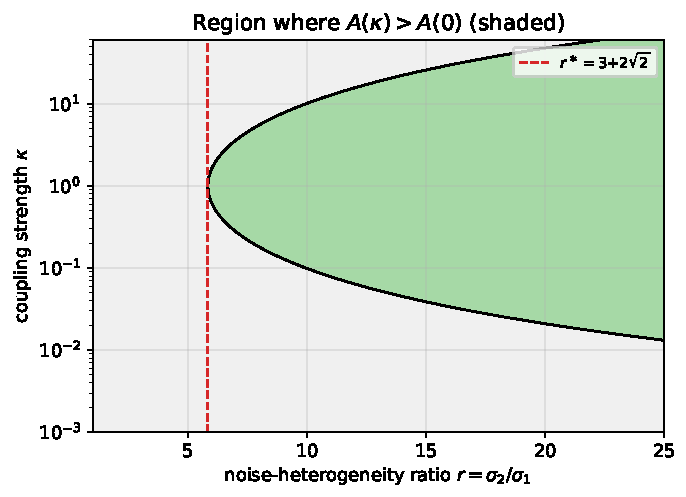
\includegraphics[width=0.85\textwidth]{figures/fig4.pdf}
\caption{Region in the $(r,\kappa)$ plane for which $A(\kappa)>A(0)$. The enhancement region
opens at the exact threshold $r=3+2\sqrt2$.}
\label{fig:4}
\end{figure}

\clearpage

\section{Strong-Coupling Limit of the Covariance Geometry}\label{sec:strong}

For $a_1=a_2=1$, $\sigma_1=1$, $\sigma_2=r$, the covariance components reduce to
\begin{align}
  \Sigma_{xx}&=\frac{\kappa^2r^2+\kappa^2+4\kappa+2}{4(2\kappa^2+3\kappa+1)}, \label{eq:sxx2}\\
  \Sigma_{yy}&=\frac{\kappa^2r^2+\kappa^2+4\kappa r^2+2r^2}{4(2\kappa^2+3\kappa+1)}, \label{eq:syy2}\\
  \Sigma_{xy}&=\frac{\kappa(r^2+1)}{4(2\kappa+1)} . \label{eq:sxy2}
\end{align}

\begin{proposition}[Strong-coupling asymptotics]\label{prop:asym}
As $\kappa\to\infty$,
\begin{equation}
  1-\rho^2(\kappa)\sim\frac{2}{\kappa},
  \qquad
  D(\kappa)\sim\frac{r^2+1}{4\kappa},
  \qquad
  A(\kappa)\sim\frac{(r^2+1)^2}{32\kappa}, \label{eq:asym}
\end{equation}
while $\Sigma_{xx},\Sigma_{yy},\Sigma_{xy}\to\dfrac{r^2+1}{8}$.
\end{proposition}

Thus $x-y$ becomes increasingly suppressed and the covariance ellipse collapses toward the line
$x=y$. In the modal form of Eq.~\eqref{eq:Amodal} this is transparent: the longitudinal
variance $\widetilde\Sigma_{11}=(1+r^2)/4$ is independent of $\kappa$, while the transverse
variance $\widetilde\Sigma_{22}$ decays like $1/(2\kappa)$ and the modal correlation like
$1/\kappa$.

\begin{remark}[On the word ``synchronization'']\label{rem:synch}
The title and the phrase ``synchronization collapse'' need to be read in a restricted sense,
and version~1 was not explicit enough about this. Three points.

First, the collapse described here is a property of the \emph{stationary covariance ellipse},
not of trajectories. The full mathematical state space remains two-dimensional for every finite
$\kappa$, the stationary Gaussian retains full support on $\mathbb{R}^2$ for every finite
$\kappa$, and $x(t)\neq y(t)$ almost surely at every time. Nothing here is synchronization in
the sense of trajectories converging.

Second, the limit is singular: $\Sigma(\kappa)$ becomes rank-deficient only as
$\kappa\to\infty$. ``Dimensional collapse'' refers to that limit, and to the fact that the
variance transverse to $x=y$ vanishes at rate $1/\kappa$, not to a literal reduction of
state-space dimension at any finite coupling.

Third, the relation to the master-stability literature \cite{PecoraCarroll1998} is geometric
only. That framework asks whether a synchronization manifold of a nonlinear system is
transversally stable; here the linear system has a globally attracting stationary distribution
for every $\kappa\ge0$, there is no stability transition, and the transverse direction is
always stable. What is shared is the decomposition into a longitudinal and a transverse mode
relative to $x=y$ --- and, as Section~\ref{sec:normalmodes} shows, even that decomposition
behaves differently here, because heterogeneous noise correlates the two modes.

A more literal description of the phenomenon would be \emph{strong-coupling degeneration of the
stationary covariance toward the diagonal}. We retain the shorter phrase in the title, for
continuity with version~1, with this remark as its definition.
\end{remark}

\section{Machine-Checked Verification}\label{sec:lean}

The central algebraic content of this paper has been formalized and machine-checked in Lean~4
with mathlib. The development is public at
\url{https://github.com/innerlightr-wq/ou-threshold-lean}; the state corresponding to this
version of the paper is recorded there as frozen snapshots under \texttt{verified/}, each with
its own toolchain file, dependency manifest, SHA-256 manifest, and build log.

\paragraph{What is formalized.} The formalization works at the level of \emph{exact real
algebra}: the stationary covariance is \emph{defined} by the closed forms
\eqref{eq:Sxx}--\eqref{eq:Sxy} in the equal-relaxation normalization, and the Lyapunov equation
is then \emph{proved} to hold for it. Specifically, the following are machine-checked:

\begin{enumerate}\itemsep2pt
\item $M\Sigma+\Sigma M^{\top}=-Q$ for the stated $\Sigma$, for all $\kappa\ge0$ and all $r$
  (\texttt{cov\_lyapunov}), together with uniqueness of the solution
  (\texttt{lyapunov\_unique}) and $\det\Sigma=A(\kappa)$ (\texttt{det\_cov}).
\item Theorem~\ref{thm:volume}, in the form
  $(\exists\,\kappa>0,\ A(\kappa,r)>A(0,r))\iff r>3+2\sqrt2$ for $r\ge1$
  (\texttt{exists\_volume\_improvement\_iff\_threshold}), including the discriminant
  factorization~\eqref{eq:discA}.
\item Proposition~\ref{prop:resid}, in the form
  $(\exists\,\kappa>0,\ D(\kappa,r)>D(0,r))\iff r>2+\sqrt3$ for $r\ge1$
  (\texttt{exists\_residual\_improvement\_iff\_threshold}), including the
  factorization~\eqref{eq:discD}.
\item The tangency~\eqref{eq:tangency} at $r=\rA$ with double root $\kappa=1$, and
  $A(\kappa,\rA)\le A(0,\rA)$ for all $\kappa\ge0$ (Corollary~\ref{cor:sub} at the boundary).
\item The reciprocal relations~\eqref{eq:s64} and $w(r^2)=s(r)^2-2$, and
  Theorem~\ref{thm:cross}: the closed form~\eqref{eq:mergerinv}, the value $J_2=16$, the
  eigenvalue ratio $q=7+4\sqrt3=(\rD)^2$, the non-vacuity of that statement (the matrix really
  has two distinct real eigenvalues), and the rapidity form~\eqref{eq:rapidity}.
\item The $n\ge3$ counterexample $(1,8,12)$ versus $(2,3,16)$.
\end{enumerate}

Each statement is checked by Lean's kernel and depends only on the three standard axioms of
mathlib's classical foundation (\texttt{propext}, \texttt{Classical.choice},
\texttt{Quot.sound}); \texttt{\#print axioms} output is included in the snapshots. There are no
\texttt{sorry}s and no appeals to \texttt{native\_decide}.

\paragraph{What is not formalized.} This is a companion to the paper, not a formalization of
it, and the gap should be stated plainly. Not formalized are: the stochastic-process content of
Proposition~\ref{prop:stationary} (existence and uniqueness of the stationary Gaussian measure
for a Hurwitz linear SDE, which is quoted from the literature and used to justify the Lyapunov
equation, not derived in Lean); the general-rate covariance~\eqref{eq:Ageneral} and
Proposition~\ref{prop:Aprime}, which are proved here by hand and checked with computer algebra
only; the monotonicity of coherence (Proposition~\ref{prop:mono}); the strong-coupling
asymptotics (Proposition~\ref{prop:asym}); the numerical table; and the figures. Formalizing
Proposition~\ref{prop:stationary} would require a treatment of linear SDEs that, to our
knowledge, mathlib does not currently have.

In short: the machine-checked part is exactly the algebra that carries the two thresholds and
the identity between them. The modelling step --- that this $\Sigma$ is the stationary
covariance of that stochastic process --- is classical, and is assumed rather than verified.

\section{Relation to the Dissipative Bosonic Josephson Junction}

An earlier study of a phenomenologically damped bosonic Josephson junction found an exact
separation between local contraction information and global basin accessibility
\cite{DeJesus2026bjj}. In that model $\tr J=-\gamma$ throughout the interior phase space, so the
local phase-space contraction rate is independent of the interaction parameter $\Lambda$, while
the measured global trapped-basin fraction varies substantially with $\Lambda$. The
conservative system also exhibits two different robustness measures with different qualitative
behavior: the energy separation is monotonic while the directional separatrix width possesses
an interior maximum.

The present OU calculation is not dynamically equivalent to that system. The common lesson is
methodological:
\begin{quote}
Exact local information can be insufficient to determine global parameter-dependent geometry,
and distinct scalar measures of the same system need not identify the same structural
threshold.
\end{quote}

The present paper strengthens the second part of that observation by producing two exact
heterogeneity thresholds, $\rD=2+\sqrt3$ for conditional residual variance and
$\rA=3+2\sqrt2$ for stationary covariance volume --- and, in Theorem~\ref{thm:cross}, by
showing that in this model the two are nonetheless algebraically related.

\section{A Provisional Intermediate Interaction Regime}

For chosen thresholds $d_0,c_0>0$, one could define
\begin{equation}
  \mathcal{C}=\bigl\{\kappa>0:\ A(\kappa)>A(0),\ D(\kappa)\ge d_0,\ C(\kappa)\ge c_0\bigr\}.
  \label{eq:regime}
\end{equation}
Such a set can be interpreted as an intermediate interaction regime satisfying simultaneous
requirements of stationary volume enhancement, retained residual structure, and nonzero
coherence. We do not elevate this definition to a theorem because $d_0$ and $c_0$ are
externally chosen.

The exact results requiring no arbitrary thresholds are instead $\rD=2+\sqrt3$,
$\rA=3+2\sqrt2$, the identity $\kappa_1\kappa_2=1$, Theorem~\ref{thm:cross}, and the strict
monotonicity of $C(\kappa)$.

\section{Limitations}\label{sec:limitations}

Several limitations are essential. Items 1--7 restate version~1; items 8--11 are new.

\begin{enumerate}\itemsep2pt
\item The model is linear, Gaussian, two-dimensional, and driven by independent additive white
  noise.
\item The principal volume threshold $3+2\sqrt2$ is proved only for equal intrinsic relaxation
  rates. Proposition~\ref{prop:Aprime} is the only general-rate result in the paper.
\item The residual threshold $2+\sqrt3$ is likewise derived in the equal-relaxation
  normalization.
\item The stationary distribution has full support in $\mathbb{R}^2$ for every finite $\kappa$,
  so $A(\kappa)$ measures covariance volume rather than mathematical reachability or support.
\item The model possesses a unique stationary state and therefore does not address multistable
  basin geometry.
\item The threshold values are properties of this model. No universal physical significance is
  attributed to either algebraic constant.
\item No inference is made from these calculations to consciousness, artificial intelligence,
  biological evolution, social systems, or cosmology.
\item The word ``synchronization'' is used in the restricted sense of
  Remark~\ref{rem:synch}: degeneration of the stationary covariance toward the diagonal in a
  singular limit. No trajectory-level or stability-theoretic synchronization statement is made
  or implied, and the master-stability framework is not applicable to this system.
\item ``Expansion'' means an increase of $\det\Sigma$ relative to its uncoupled value at the
  same parameters. It is a statement about second moments of a Gaussian measure with fixed full
  support, and it is bounded: by Proposition~\ref{prop:asym}, $A(\kappa)\to0$, so any
  enhancement is a transient of the coupling parameter, not a persistent gain.
\item Theorem~\ref{thm:cross} is an exact identity, verified symbolically and mechanically, but
  it is an identity within one two-parameter family. We have not derived it from a structural
  principle, we do not claim it generalizes, and the $n\ge3$ counterexample above shows that
  the invariant it is built from does not by itself survive to larger networks.
\item The formalization of Section~\ref{sec:lean} verifies algebra, not modelling. In
  particular, no part of the stochastic-process argument is machine-checked, and a reader who
  doubts Proposition~\ref{prop:stationary} gains nothing from the Lean development.
\end{enumerate}

\section{Nonlinear Bistable Extension}

A natural falsification test is a pair of coupled stochastic bistable systems:
\begin{align}
  dx &= -V_1'(x)\,dt+\kappa(y-x)\,dt+\sigma_1\,dW_1, \label{eq:bist1}\\
  dy &= -V_2'(y)\,dt+\kappa(x-y)\,dt+\sigma_2\,dW_2, \label{eq:bist2}
\end{align}
with $V_i(x)=\dfrac{x^4}{4}-\dfrac{a_ix^2}{2}$.

Each uncoupled subsystem possesses two metastable wells, giving four coarse joint
configurations: $(--)$, $(-+)$, $(+-)$, $(++)$. This system can test whether an intermediate
coupling regime preserves mixed configurations while modifying transition structure, and
whether strong coupling suppresses the mixed states in favor of synchronized configurations.
No results for this nonlinear extension are reported here.

\section{Companion Note: A General Two-Mode Reduction}\label{sec:companion}

The volume threshold of Section~\ref{sec:volume} turns out not to depend on the graph at all,
but only on a two-dimensional reduction, and a machine-checked account of this is included in
the companion repository (module \texttt{ActivePlane}). Briefly: let a Hurwitz drift have a
two-dimensional invariant plane with decay rates $D_1,D_2>0$, and let the forcing be a rank-one
deformation of the isotropic one, $Q=q_b\bigl(I+(\tau-1)ee^{\top}\bigr)$, where $e$ is a unit
\emph{excitation direction} (the direction along which the forcing is anisotropic; $e$ here is
never Euler's number) making an angle with the drift eigenbasis given by $e=cu+sv$,
$c^2+s^2=1$. Then the stationary covariance in that plane satisfies the palindromic determinant
identity $4D_1D_2\det\Sigma=q_b^2\bigl(\mathcal{A}\tau^2+(1-2\mathcal{A})\tau+\mathcal{A}\bigr)$
with $\mathcal{A}=c^2s^2\nu^2$ and $\nu=(D_1-D_2)/(D_1+D_2)$; dividing by $\tau$ gives
$1+\mathcal{A}\bigl(w(\tau)-2\bigr)$ with $w$ as in Eq.~\eqref{eq:sw}. The palindromic
structure is the self-duality $Q_e(\tau)=\tau\,Q_{e^{\perp}}(1/\tau)$, which holds because
$ee^{\top}+e^{\perp}e^{\perp\top}=I$; this is why a reciprocal invariant appears at all, and it
explains why the relevant reciprocal variable is the \emph{variance} ratio $\tau=r^2$ rather
than the amplitude ratio. The present paper's threshold is the instance $\tau=r^2$,
$w=34$, of that identity. A separate write-up of the general statement is in preparation and is
not part of this version.

\section{Strongest Defensible Contribution}

The principal exact contribution can be summarized as follows.

\begin{quote}
For two diffusively coupled Ornstein--Uhlenbeck processes with equal relaxation rate, the
stationary covariance volume $A(\kappa)=\det\Sigma(\kappa)$ always satisfies $A'(0)<0$.
Nevertheless, $\sup_{\kappa>0}A(\kappa)>A(0)$ if and only if
$\max(\sigma_1/\sigma_2,\sigma_2/\sigma_1)>3+2\sqrt2$. When the enhancement regime exists, its
two boundary couplings satisfy $\kappa_1\kappa_2=1$. Separately, the conditional residual
variance can exceed its uncoupled value if and only if the noise-amplitude ratio exceeds
$2+\sqrt3$. Gaussian coherence increases strictly with coupling for every positive noise ratio.
Both thresholds are reciprocal units, $s(\rA)=6$ and $s(\rD)=4$; and at the coupling
$\kappa=1$ where the volume enhancement region degenerates, the covariance eigenvalue ratio is
exactly $(\rD)^2=7+4\sqrt3$.
\end{quote}

The two distinct thresholds demonstrate exactly that covariance-volume expansion, retained
residual distinction, and coherence are not interchangeable measures, even though all three
arise from the same covariance matrix. That they are nonetheless algebraically related, in the
precise sense of Theorem~\ref{thm:cross}, is the main new result of this version.

\section{Conclusion}

Two diffusively coupled OU processes provide a minimal analytically solvable setting in which
heterogeneity, coupling, coherence, and covariance geometry can be separated exactly.

The first result is universal: $A'(0)<0$. Infinitesimal coupling always contracts stationary
covariance volume.

The global response, however, depends on heterogeneity. In the equal-relaxation model,
$\exists\,\kappa>0:A(\kappa)>A(0)$ if and only if $r>3+2\sqrt2$. A distinct and lower
threshold, $r>2+\sqrt3$, governs enhancement of conditional residual variance. Both are
reciprocal units, and they meet at the critical coupling in the sense of
Theorem~\ref{thm:cross}. Meanwhile $C(\kappa)$ increases monotonically for all positive $r$,
while sufficiently strong coupling drives $\rho\to1$, $D\to0$, $A\to0$.

The resulting picture is therefore not that coupling is generically enriching. Rather,
sufficiently heterogeneous systems in this particular model can exhibit a bounded intermediate
range in which stationary covariance volume exceeds its uncoupled value before the stationary
covariance ultimately degenerates toward the diagonal. Whether an analogous architecture
survives in nonlinear and multistable systems remains an open question.

\section*{Acknowledgments}
\addcontentsline{toc}{section}{Acknowledgments}

AI assistance (Anthropic's Claude, used through Claude Code) was used for symbolic algebra
verification, numerical computation, literature search and citation verification, construction
and checking of the Lean~4 formalization reported in Section~\ref{sec:lean}, and manuscript
preparation, including the reconstruction of this document from the version~1 PDF described in
Section~0. Every mathematical statement retained from version~1 was re-derived symbolically
before being carried over, and the statements listed in Section~\ref{sec:lean} are in addition
checked by Lean's kernel, which does not depend on the assistant's correctness. All conceptual
development, research direction, interpretation, and final responsibility for the work remain
with the author.

\appendix

\section{Reproducibility}

All symbolic derivations and numerical results were independently checked using Python with
SymPy, NumPy, and SciPy. The explicit stationary covariance solution was compared with the
independent numerical solver \texttt{scipy.linalg.solve\_continuous\_lyapunov} at multiple
parameter points. The maximum observed elementwise discrepancy was approximately
$2.8\times10^{-14}$.

The reproducibility script accompanying this manuscript verifies:
\begin{enumerate}\itemsep1pt
\item the exact Lyapunov solution;
\item Proposition~\ref{prop:Aprime};
\item the difference formula, Eq.~\eqref{eq:diff};
\item the discriminant factorization, Eq.~\eqref{eq:discA};
\item the threshold $3+2\sqrt2$;
\item the reciprocal identity $\kappa_1\kappa_2=1$;
\item the residual-variance threshold $2+\sqrt3$;
\item the exact positivity factorization for $d\rho^2/d\kappa$;
\item the strong-coupling asymptotics;
\item the numerical table and figures.
\end{enumerate}

New in this version, and checked the same way before being stated: the modal
form~\eqref{eq:Amodal} and its identity with Eq.~\eqref{eq:Aequal}; the merger
invariant~\eqref{eq:mergerinv}; and the values in Table~\ref{tab:invariants}. These, together
with the statements listed in Section~\ref{sec:lean}, are in addition machine-checked in
Lean~4.

\section{Note on the figures in this version}

The figures of version~1 were reproduced in this version by extracting the four vector graphics
from the deposited version~1 PDF, without modification of their content. They are therefore
identical to the version~1 figures and were not regenerated. The script that originally
produced them was not preserved with the manuscript source; see Section~0.

\bibliographystyle{plain}
\bibliography{../../references}

\end{document}
